\subsection{Optoelectronic Materials}

Optoelectronic materials convert light to electric energy and/or electric energy to light. The study of these materials goes back as far as the early 1900s, but accelerates rapidly in the 1960s with the advent of the light emitting diode and semiconductor laser \cite{sweeney_optoelectronic_2017}. Optoelectronic devices are ubiquitous; they have enabled the rapid growth of information technologies around the world, and are fundamental in modern telecommunication and internet infrastructure. Modern optronics research explores new materials that can be used to create faster, more efficient, and smaller optoelectronic devices.

\subsubsection{Organic Photovoltaic: ADT}

Organic optoelectronic materials are not a new discovery, but have become increasingly popular in recent decades as methods for creating them have advanced \cite{ostroverkhova_organic_2016}. The Ostroverkhova group at Oregon State University have studied several organic photovoltaics (OPVs) including functionalized derivatives of pentacene, benzothiophene, and anthradithiophene (ADT) \cite{shepherd_optical_2010, e._b._shepherd_effect_2011, platt_optical_2009}. A drop-cast sample of fluorinated ADT with triethylsilyethynyl (TES) functional group, provided by the Ostroverkhova group, is used for demonstration of the new microspectrometer device in Chapter \ref{chap:results}.

\begin{figure}[H]
    \centering
    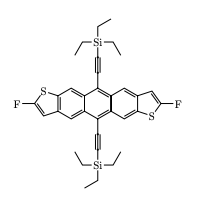
\includegraphics{img/adt-tes-f.png}
    \caption[Molecular diagram of ADT TES-F.]{Molecular diagram of fluorinated anthradithiophene (ADT) with triethylsilyethynyl (TES) side group. A drop-cast sample of this molecule was provided by the Ostroverkhova group at Oregon State University, and used for demonstration of our microspectrometer instrument following a study by Lam \cite{lam_polarization_2018}. Diagram from Shepherd \emph{et al.} \cite{shepherd_optical_2010}.}
    \label{fig:adt-diagram}
\end{figure}

\subsubsection{Quantum Dots: \ce{CdSe}}

Quantum dots (QDs) are artificial semiconductor particles. They are typically only a few nanometers in size, and there has been a fair amount of research on the tunability of optoelectronic properties in QDs by varying their size and shape. Quantum dots have many of the same potential applications as other optoelectronic materials, but are attractive for their size and reproducibility. Previous studies have shown how quantum dots can be produced en masse, with a high degree of control over their shape and size \cite{empedocles_photoluminescence_1996, murray_synthesis_2000}.

A sample of CdSe quantum dots, suspended in solution and drop-cast on a glass slide, is used to demonstrate the new microspectrometer device in Chapter \ref{chap:results}.

\subsection{Mechanics of Photoluminescence}
/note{Should I even bother?}

% Photoluminescence (PL) is a mechanism by which materials absorb and emit photons. The process can be described with respect to electronic transitions within an atom or molecule.

% The absorptive transition occurs first, when a photon interacts with a molecule and is absorbed. The photon's energy must be approximately equal to the bandgap of the absorbing molecule to satisfy the energy transitions allowed by quantum mechanics. When that condition is met, the photon's energy raises an electron to an excited state, where it stays for a short time.

% Some number of vibronic transitions occur as the electron loses energy to radiation and vibration. \todo{How do we measure these transitions, or their lifetimes?}

% Finally, the radiative transition occurs when the electron decays back to a ground state. During the radiative transition, a photon is emitted at the bandgap energy as the electron moves from the lowest vibronic state in the conduction band to the highest vibronic state in the valence band. \todo{This needs some work.}

% \todo{Why is PL a useful measurement in solid state? In biological sciences? In general?}
